\documentclass[a4paper,12pt]{report}

\usepackage[utf8]{inputenc}
\usepackage[T1]{fontenc}
\usepackage[margin=2.5cm]{geometry}
\usepackage{setspace}
\usepackage{graphicx}
\usepackage{amsmath}
\usepackage{booktabs}
\usepackage{float}
\usepackage{placeins}
\usepackage{caption}
\usepackage[hidelinks]{hyperref}
\usepackage[round]{natbib}
\usepackage{tikz}
\usetikzlibrary{shapes.geometric, arrows.meta, positioning}

\setlength{\parskip}{0.5em}
\setlength{\textfloatsep}{10pt}
\onehalfspacing



\begin{document}

\begin{titlepage}
\centering

\vspace*{0cm}
\includegraphics[width=0.4\textwidth]{maps/logo_unibo.png}

\vspace{0.5cm}

{\large DEPARTMENT OF BIOLOGICAL, GEOLOGICAL AND ENVIRONMENTAL SCIENCES (BIGEA)}

\vspace{1cm}

{\large SECOND CYCLE DEGREE IN}

{\large SCIENCES AND MANAGEMENT OF NATURE}

{\large GLOBAL CHANGE ECOLOGY AND SUSTAINABLE DEVELOPMENT GOALS}

\vspace{1cm}

{\LARGE \textbf{MINING-INDUCED FOREST DEGRADATION IN GHANA'S PRA RIVER BASIN: A MULTI-TEMPORAL REMOTE SENSING ANALYSIS} \par}

\vspace{1cm}

{\large Dissertation in Spatial Ecology in R}

\vspace{1cm}

\noindent
\begin{minipage}[t]{0.45\textwidth}
\raggedright
\textbf{Supervisor} \\
Prof. Duccio Rocchini
\end{minipage}
\hfill
\begin{minipage}[t]{0.45\textwidth}
\raggedleft
\textbf{Defended by} \\
Iris Nana Obeng
\end{minipage}

\vspace{1cm}

\noindent\rule{\textwidth}{0.6pt}

{\large Graduation Session: July 2026}

{\large Academic Year 2025/2026}

\end{titlepage}


\chapter*{Acknowledgements}
\addcontentsline{toc}{chapter}{Acknowledgements}

\setlength{\parindent}{0pt}    
\setlength{\parskip}{0.5\baselineskip}  

I would like to express my sincere gratitude to Professor Duccio Rocchini for his guidance, encouragement, and invaluable support throughout this research. I am especially grateful for the opportunity to contribute to research activities under his supervision prior to the commencement of this thesis. This experience provided valuable exposure to spatial ecology and remote sensing research, and helped develop the skills and confidence that contributed significantly to the successful completion of this study.

I would also like to express my sincere appreciation to my course mate, Sofia Bissoni, for her support and encouragement during the Spatial Ecology course. Her willingness to share knowledge and provide guidance greatly enriched my learning experience and gave me the confidence to engage fully with the course and undertake the examination. Through that experience, I was able to further develop my interest in spatial ecology and demonstrate my commitment to the subject.

I am also grateful to the Department of Biological, Geological and Environmental Sciences (BIGEA), University of Bologna, for providing an enriching academic environment and the resources necessary to undertake this research.

Finally, I acknowledge the Copernicus Programme of the European Union for providing free access to Sentinel-2 satellite imagery, which formed the basis of this research.

\setlength{\parindent}{15pt}    
\setlength{\parskip}{0pt}        

 
\begin{abstract}

Mining-induced forest degradation is an increasing environmental concern in tropical regions due to the expansion of both artisanal and large-scale mining activities. In Ghana, the Pra River Basin has experienced significant environmental pressure resulting from loss of vegetation, land disturbance, and ecosystem degradation associated with gold mining. Effective approaches are therefore required to monitor changes in forest condition and identify the spatial extent of mining-related environmental impacts.

This study assessed mining-induced forest degradation within the Pra River Basin using a multi-temporal remote sensing approach based on Sentinel-2 satellite imagery acquired in 2018, 2020, and 2022. The analysis integrated NDVI-based land-cover classification, fuzzy classification, and spectral distance analysis to evaluate changes in vegetation condition over time and detect areas affected by mining-related disturbances.

The results showed a progressive decline in vegetation condition in the study area, with the largest reductions observed between 2020 and 2022. NDVI change detection indicated that approximately 29.3\% of the study area experienced vegetation decline, while only 1.7\% showed vegetation recovery. Spectral distance analysis also revealed an increase in spectral divergence from reference forest conditions in areas surrounding mining-influenced zones, suggesting gradual ecological deterioration.

The findings suggest that combining NDVI with spectral distance analysis provides a more comprehensive approach for detecting both direct forest loss and subtle changes in vegetation condition than single-index approaches alone. The study contributes to understanding the environmental change related to mining in Ghana and demonstrates the usefulness of integrated remote sensing methods to monitor forest degradation in tropical landscapes.

\textbf{Keywords:} Forest degradation; Mining-related disturbance; Remote sensing; NDVI; Spectral distance analysis; Sentinel-2; Pra River Basin; Ghana.

\end{abstract}

\tableofcontents
\listoffigures
\listoftables
\clearpage
\pagenumbering{arabic}

\chapter{Introduction}

\section{Background to the Study}

Mining-induced forest degradation has become one of the most significant environmental challenges in tropical regions \citep{asner2005selective,sonter2017mining}. The expansion of large-scale and artisanal mining often leads to the removal of vegetation, the exposure of bare soil, the fragmentation of habitats, and the deterioration of river systems. In many developing countries, these impacts are intensified by weak environmental regulation and the rapid growth of informal mining activities. Tropical forests are particularly vulnerable because mining commonly occurs along river valleys and floodplains where vegetation is dense and mineral deposits are abundant.

Across West Africa, mining has increasingly transformed forest landscapes. The conversion of vegetated land into mining pits, spoil heaps, and access roads contributes to long-term ecological degradation. In addition to direct forest loss, mining often produces more subtle forms of degradation, including canopy thinning, reduced vegetation health, and gradual changes in forest structure. These effects may occur long before complete forest clearance is visible \citep{tarazona2020monitoring}.

Ghana is one of the leading gold-producing countries in Africa, and the mining sector contributes significantly to national income and employment \citep{bansah2016hazardous,mcquilken2016asm}.
However, the rapid expansion of both legal and illegal mining has generated serious environmental concerns \citep{hilson2002land,hilson2002environmental}. Informal mining, locally known as ``galamsey'', has become widespread in many parts of the country, particularly within forested and riverine areas. Numerous studies have reported that mining activities in Ghana are associated with deforestation, water pollution, river sedimentation, and loss of biodiversity \citep{mcquilken2016asm,forkuor2012comparison,bansah2016hazardous,barenblitt2021ghana}. Recent remote sensing studies further show that artisanal and small-scale mining has become a major driver of vegetation loss across mining regions of Ghana, contributing substantially to landscape degradation and forest disturbance \citep{barenblitt2021ghana}.

The Pra River Basin is among the most affected landscapes in Ghana. The basin drains parts of the Ashanti, Eastern, and Central Regions before flowing into the Gulf of Guinea. It contains extensive tropical forest cover, fertile agricultural land, and major river systems that support local livelihoods. At the same time, the basin is rich in gold deposits, making it an important centre of both artisanal and large-scale mining. Over the past decade, increasing mining activity within the basin has accelerated vegetation removal and degraded surrounding forest ecosystems. Previous remote sensing investigations within the Pra River Basin have documented substantial land-cover change associated with gold mining, urban expansion, and agricultural development, highlighting the growing environmental pressure within the basin \citep{awotwi2018pra}.

Despite the growing concern over environmental degradation in the Pra River Basin, there is still limited understanding of how mining has altered forest condition over time. Most previous studies have focused primarily on general land-cover change or on the distribution of mining sites. Fewer studies have attempted to measure the progressive degradation of forest areas surrounding mining-influenced zones. Consequently, there is a need for approaches that not only identify where mining-related disturbance is occurring, but also evaluate the extent to which forest condition is changing.

Remote sensing provides an effective means of addressing this problem because it allows land-cover changes to be monitored repeatedly over large areas and over long periods of time \citep{lu2004change,singh1989review}. The Normalized Difference Vegetation Index (NDVI) is widely used to assess vegetation condition because it is sensitive to differences between red and near-infrared reflectance \citep{tucker1979ndvi}. Healthy vegetation typically produces high NDVI values, while bare soil, mining-related surfaces, and degraded vegetation tend to produce lower values. However, NDVI alone may not capture the early stages of forest degradation, especially where vegetation remains partially intact.

To overcome this limitation, spectral distance analysis can be combined with NDVI-based classification. Spectral distance methods measure the similarity between observed pixels and a reference forest condition. As forest areas become increasingly disturbed, their spectral properties diverge from those of intact forest. Integrating NDVI and spectral distance analysis therefore provides a more comprehensive framework for identifying both direct forest loss and more gradual forms of mining-related degradation.

This study applies such an approach to the Pra River Basin using Sentinel-2 satellite imagery from 2018, 2020, and 2022. The study combines NDVI-based land-cover classification with spectral distance metrics in order to assess changes in forest condition and identify the influence of mining-related disturbance over time.


\section{Problem Statement}

The Pra River Basin has experienced increasing pressure from both artisanal and large-scale gold mining. Although mining contributes to economic development, its expansion has been associated with widespread environmental degradation. Forest cover has been removed in many areas, while remaining vegetation has become increasingly fragmented and disturbed. River systems within the basin have also been affected through sedimentation and pollution.

Existing research in the Pra River Basin has largely concentrated on mapping general land-use and land-cover change. While such studies are useful, they do not fully capture the progressive degradation of forest ecosystems surrounding mining-influenced areas. In particular, conventional land-cover classifications may identify areas that have already been converted to mining land, but they often fail to detect more subtle changes in forest condition occurring before complete clearance.

Furthermore, many previous studies rely exclusively on NDVI or similar vegetation indices. Although NDVI is effective for distinguishing vegetated and non-vegetated surfaces, it may underestimate degradation where vegetation remains present but has become spectrally altered. As a result, there is a need for a method that can identify both clear land-cover change and more gradual deterioration in forest condition.

This study addresses that gap by integrating NDVI-based classification with spectral distance analysis. Through this approach, the study seeks to determine how forest condition within the Pra River Basin has changed between 2018 and 2022 and to evaluate the extent to which those changes are associated with mining-related disturbance.

\section{Aim of the Study}

The aim of this study is to assess mining-induced forest degradation in Ghana's Pra River Basin using a multi-temporal remote sensing approach based on NDVI classification and spectral distance analysis.

\section{Specific Objectives}

The specific objectives of the study are:

\begin{itemize}
\item To map vegetation condition and mining-related land-cover classes in the Pra River Basin using NDVI thresholds.
\item To identify areas of likely mining-related disturbance by analysing changes in vegetation condition between 2018 and 2022.
\item To quantify forest degradation using spectral distance metrics derived from Sentinel-2 imagery.
\item To evaluate the usefulness of combining NDVI and spectral distance analysis for monitoring mining-induced forest degradation.
\end{itemize}

\section{Research Questions}

\begin{itemize}
\item How has vegetation condition changed in the Pra River Basin between 2018 and 2022?
\item Where are mining-related land-cover changes concentrated within the basin?
\item To what extent has forest spectral condition diverged from reference forest signatures over time?
\item Can the integration of NDVI and spectral distance analysis provide a more effective approach for detecting mining-induced forest degradation?
\end{itemize}


\section{Significance of the Study}

The study is important for both environmental management and remote sensing research. From an environmental perspective, the findings provide evidence of how mining-related activities are associated with forest ecosystem changes within the Pra River Basin. Such information can support government agencies, environmental organizations, and policy makers in identifying areas where intervention and restoration are most urgently needed.

The study is also significant because it demonstrates the value of combining NDVI and spectral distance analysis. While NDVI is widely used in vegetation monitoring, the addition of spectral distance metrics provides a more detailed understanding of forest degradation. The integrated approach developed in this study may therefore be useful for monitoring mining-related impacts in other tropical regions where gradual forest degradation is difficult to detect.

Finally, the study contributes to the growing body of research on the environmental consequences of mining in Ghana. By focusing specifically on the Pra River Basin and examining change across multiple years, the study provides a clearer picture of the temporal progression of mining-related forest degradation.

\section{Scope of the Study}

The study is limited to the approximate extent of the Pra River Basin in southern Ghana. The analysis focuses on changes occurring between 2018 and 2022 using Sentinel-2 imagery acquired during the dry season. The study examines vegetation condition, mining-related land-cover change, and forest spectral degradation within the selected area.

The research is restricted to satellite-based analysis and does not include field verification or direct measurements of forest condition. Consequently, the results should be interpreted as an assessment of relative patterns of vegetation and landscape change rather than an exact measurement of on-the-ground ecological conditions.

\section{Organization of the Thesis}

The thesis is organized into seven chapters.

Chapter One introduces the study and presents the problem statement, objectives, research questions, significance, and scope of the research.

Chapter Two reviews relevant literature on mining-induced forest degradation, remote sensing of vegetation change, NDVI, and spectral distance analysis.

Chapter Three describes the study area.

Chapter Four outlines the datasets and methodological procedures used in the analysis.

Chapter Five presents the results of the NDVI and spectral distance analyses.

Chapter Six discusses the findings.

Chapter Seven presents the conclusions and recommendations.


\chapter{Literature Review}

Mining-induced forest degradation has become a major environmental concern in many tropical regions due to the rapid expansion of mineral extraction activities and the increasing pressure placed on forest ecosystems. In recent decades, the growth of small-scale and artisanal mining activities has intensified environmental degradation in many developing countries, particularly in areas characterized by high biodiversity and ecologically sensitive landscapes. Forest ecosystems located near mining zones frequently experience vegetation removal, soil disturbance, habitat fragmentation, and water pollution, resulting in long-term ecological consequences.

The increasing environmental impacts associated with mining-related activities have created a growing need for effective monitoring approaches capable of identifying both direct land-cover change and gradual ecological degradation. Conventional field-based environmental assessments are often limited by cost, accessibility, and temporal constraints, particularly in tropical environments where vegetation cover is dense and large areas are difficult to access. Consequently, remote sensing has emerged as an important tool for environmental monitoring because it allows large-scale vegetation analysis to be conducted efficiently over long periods of time.

This chapter reviews literature related to mining-induced forest degradation and the application of remote sensing techniques in vegetation monitoring. The chapter first discusses the environmental impacts of mining activities within tropical forest ecosystems before examining mining-related environmental change in Ghana. The review then explores the theoretical foundations and applications of remote sensing appro,aches including the Normalized Difference Vegetation Index (NDVI), spectral distance analysis, and Sentinel-2 imagery. Finally, the chapter identifies gaps within existing research and explains the relevance of the present study.


\section{Forest Degradation in Tropical Environments}

Forest degradation refers to the reduction in the ecological quality, productivity, and structural integrity of forest ecosystems without necessarily resulting in complete forest removal. Unlike deforestation, which involves total conversion of forest land to non-forest land uses, forest degradation often occurs gradually through processes that reduce vegetation health and alter ecosystem functioning.

Tropical forests are among the most biologically diverse ecosystems in the world and provide essential ecological services including carbon sequestration, biodiversity conservation, climate regulation, and hydrological stability. However, these ecosystems are increasingly threatened by human activities such as agricultural expansion, logging, infrastructure development, and mining-related activities \citep{asner2005selective,sonter2017mining}.

Mining activities represent one of the most environmentally intensive drivers of forest degradation because they involve extensive land disturbance and often occur within ecologically sensitive areas \citep{hilson2002land}. Surface mining operations frequently require the clearing of vegetation, excavation of soil, and alteration of drainage systems, all of which contribute to the deterioration of surrounding ecosystems.

In many tropical regions, forest degradation associated with mining extends beyond the immediate extraction zones. Vegetation surrounding mining sites may experience increased sediment deposition, soil compaction, reduced water availability, and increased human disturbance. These impacts can gradually alter forest structure and reduce vegetation health even where complete forest removal has not occurred.

The gradual nature of mining-related degradation creates significant challenges for environmental monitoring because early stages of vegetation stress may not be easily detected using conventional land-cover classification methods. Consequently, there is increasing interest in remote sensing approaches capable of detecting both direct vegetation loss and subtle ecological deterioration \citep{richards2013remote,tarazona2020monitoring}.

\section{Mining and Environmental Degradation in Ghana}

Ghana has a long history of gold mining and remains one of the leading gold-producing countries in Africa. The mining sector contributes substantially to national economic development through employment creation, foreign exchange earnings, and government revenue generation. Despite these economic benefits, mining activities have also produced significant environmental challenges across many parts of the country \citep{hilson2002land,hilson2002environmental}.

Both large-scale industrial mining and artisanal mining operations occur within Ghana. Artisanal mining, commonly referred to as \textit{galamsey}, has expanded considerably over recent decades due to rising gold prices, unemployment, and increasing demand for mineral resources. Much of this activity occurs informally and outside effective environmental regulation \citep{mcquilken2016asm}.

Numerous studies have reported that mining activities in Ghana contribute to deforestation, river pollution, biodiversity loss, and soil degradation \citep{forkuor2012comparison,bansah2016hazardous}. River systems such as the Pra, Ankobra, Birim, and Offin Rivers have experienced severe environmental deterioration resulting from mining activities occurring along riverbanks and floodplains.

Remote sensing studies in Ghana have further demonstrated the usefulness of satellite data for monitoring land-cover change associated with mining expansion and forest disturbance. For example, studies in forest–savanna transition zones and river basins have shown that multispectral imagery can effectively capture vegetation loss and landscape modification driven by anthropogenic activities, including mining \citep{forkuor2012comparison,awotwi2018pra,gallwey2020sentinel}.

The Pra River Basin has become one of the most environmentally affected regions in Ghana because of intensive gold mining activity. Mining operations within the basin have resulted in widespread vegetation removal, degradation of riparian ecosystems, and increased sedimentation within river systems. These environmental impacts threaten both ecological stability and local livelihoods dependent on forest and water resources.

Despite growing interest in mining-related environmental change in Ghana, most previous studies have focused on either mapping mining expansion or assessing general land-cover change. Fewer studies have examined the progressive degradation of forest condition surrounding mining areas using multi-temporal remote sensing approaches. This limitation highlights the need for methods that can capture both direct land-cover conversion and gradual ecological deterioration.

\section{Remote Sensing in Environmental Monitoring}

Remote sensing refers to the acquisition of information about the Earth’s surface without direct physical contact, typically through satellite or airborne sensors. Remote sensing data sources such as Landsat and AVHRR have long been used for large-scale land-cover monitoring and environmental assessment \citep{townshend1992landsat}. Remote sensing technologies have become increasingly important in environmental monitoring because they provide repeated observations across large geographical areas and extended time periods \citep{richards2013remote,xu2013review,wulder2004forest}.

One major advantage of remote sensing is its ability to monitor inaccessible or environmentally sensitive regions where field surveys may be difficult or expensive to conduct. Multi-temporal satellite imagery allows environmental conditions to be compared across different time periods, making it possible to identify trends in land-cover and vegetation condition over time.

Vegetation monitoring represents one of the most common applications of remote sensing. Vegetation interacts with electromagnetic radiation in predictable ways, particularly within visible and near-infrared wavelengths. Healthy vegetation absorbs large amounts of red light for photosynthesis while reflecting near-infrared radiation as a result of internal leaf structure. These spectral characteristics provide the basis for many vegetation indices and classification techniques used in environmental monitoring.

Remote sensing approaches have been widely applied in studies of deforestation, wildfire assessment, agricultural monitoring, wetland mapping, and mining-related land degradation \citep{cohen1992estimating}. In Ghana, remote sensing techniques have increasingly been applied to monitor mining-related environmental change. Recent studies using satellite imagery and machine learning approaches have successfully mapped artisanal and small-scale mining activities and quantified associated vegetation loss, demonstrating the value of Earth observation data for environmental management \citep{barenblitt2021ghana,gallwey2020sentinel}. 

Recent advances in satellite technology have improved the spatial, spectral, and temporal resolution of environmental datasets. Modern satellite systems now provide high-resolution imagery suitable for detailed vegetation analysis and multi-temporal environmental assessment.


\section{Normalized Difference Vegetation Index (NDVI)}

The Normalized Difference Vegetation Index (NDVI) is one of the most widely used spectral indices in vegetation monitoring, originally developed by Rouse et al. (1974) and later refined for operational satellite applications \citep{rouse1974ndvi,tucker1979ndvi}. NDVI is designed to evaluate vegetation condition by measuring differences between red and near-infrared reflectance.

Healthy vegetation strongly absorbs visible red light for photosynthesis while reflecting substantial amounts of near-infrared radiation. In contrast, bare surfaces, water bodies, and degraded vegetation typically exhibit lower near-infrared reflectance and consequently lower NDVI values.

\begin{equation}
NDVI = \frac{NIR - Red}{NIR + Red}
\end{equation}

where \textit{NIR} represents near-infrared reflectance and \textit{Red} represents red reflectance.

NDVI values generally range between -1 and +1. Values approaching +1 indicate dense and healthy vegetation, whereas values closer to zero or negative values are associated with sparse vegetation, bare soil, or water surfaces.

NDVI has been extensively applied in studies of forest monitoring, agricultural productivity assessment, drought analysis, and environmental degradation \citep{pettorelli2011ndvi_limits}. In mining-related studies, NDVI is particularly useful for identifying vegetation loss associated with excavation, soil exposure, and land disturbance.

Despite its widespread application, NDVI also has several limitations. Because the index primarily measures vegetation greenness, it may not fully capture subtle ecological degradation where vegetation remains partially present. Disturbed forests may continue to exhibit moderate NDVI values despite experiencing canopy thinning, vegetation stress, or structural degradation. Consequently, NDVI alone may underestimate gradual forms of forest degradation.

\section{Spectral Distance Analysis}

Spectral distance analysis is a remote sensing technique used to evaluate the similarity or dissimilarity between spectral signatures. The technique is based on the assumption that different land-cover types and surface conditions across multiple wavelength bands \citep{richards2013remote}.

As forest vegetation becomes degraded, its spectral properties gradually diverge from those of healthy vegetation. Spectral distance methods therefore quantify changes in vegetation condition relative to a reference spectral signature.

One of the most commonly applied spectral distance measures is Euclidean distance, which calculates the distance between observed spectral values and a reference centroid across multiple spectral bands computed across selected bands.

\begin{equation}
D = \sqrt{(B-B_c)^2 + (G-G_c)^2 + (R-R_c)^2 + (NIR-NIR_c)^2}
\end{equation}

where:

\begin{itemize}
\item \textit{D} represents spectral distance,
\item \textit{B}, \textit{G}, \textit{R}, and \textit{NIR} represent observed spectral values,
\item \textit{B\_c}, \textit{G\_c}, \textit{R\_c}, and \textit{NIR\_c} represent the centroid values of the reference spectral class.
\end{itemize}

Lower spectral distance values indicate greater similarity to the reference condition, whereas higher values indicate increasing spectral divergence.

Spectral distance analysis is particularly useful for detecting gradual environmental change because it incorporates information from multiple spectral bands simultaneously. Unlike single-index approaches such as NDVI, spectral distance methods are capable of identifying subtle changes in vegetation condition that may not be immediately visible through vegetation greenness alone.

Previous studies have applied spectral distance analysis in the monitoring of forest degradation caused by logging, agricultural expansion, fire, and mining activities \citep{tarazona2020monitoring}. Combining spectral distance analysis with NDVI may therefore improve the detection of both direct vegetation loss and progressive ecological degradation.


\section{Sentinel-2 Imagery and Environmental Applications}

The Sentinel-2 satellite mission, developed by the European Space Agency (ESA), provides multispectral imagery suitable for environmental monitoring applications \citep{drusch2012sentinel,esa2024sentinel2}. It has become widely used in remote sensing studies because of its relatively high spatial resolution, frequent revisit cycle, and freely accessible datasets.

Sentinel-2 provides imagery across multiple spectral bands including visible, near-infrared, and shortwave infrared wavelengths. Several of these spectral bands are particularly relevant for vegetation analysis, land-cover classification, and environmental monitoring.

The satellite’s 10 m spatial resolution enables relatively detailed mapping of vegetation condition and surface disturbance. Its five-day revisit frequency also supports multi-temporal monitoring of environmental change.

Sentinel-2 imagery has been widely applied in studies of deforestation, agricultural monitoring, wildfire assessment, wetland mapping, and mining-induced environmental degradation \citep{forkuor2012comparison}. In tropical regions, Sentinel-2 imagery has proven especially useful for identifying vegetation disturbance associated with artisanal and small-scale mining. In tropical regions, Sentinel-2 imagery has proven especially useful for identifying vegetation disturbance associated with artisanal and small-scale mining. For example, Gallwey et al. \citep{gallwey2020sentinel} developed a Sentinel-2-based deep learning approach for detecting artisanal mining activities in Ghana and demonstrated the capability of Sentinel-2 imagery for monitoring mining-related deforestation and landscape disturbance.

The availability of free, high-resolution imagery makes Sentinel-2 particularly valuable in developing countries where access to commercial satellite datasets may be limited.


\section{Research Gap}

Although previous studies have investigated mining-related environmental change in Ghana, most have focused primarily on mapping mining expansion, general land-cover change, or deforestation patterns \citep{awotwi2018pra,gallwey2020sentinel}. While these studies provide valuable spatial information, they often emphasize discrete land-cover transitions rather than gradual ecological degradation processes.

Furthermore, many existing studies rely exclusively on NDVI or similar vegetation indices. Although NDVI is effective for distinguishing vegetated from non-vegetated surfaces, it may underestimate degradation in areas where vegetation remains partially intact but has experienced structural or physiological stress.

Limited research in Ghana has integrated NDVI-based classification with spectral distance analysis to evaluate both abrupt land-cover change and progressive forest degradation within mining landscapes. As a result, there remains a methodological gap in detecting early-stage ecological disturbance associated with mining activity using multi-temporal satellite data.

This study addresses this gap by integrating NDVI-based classification with fuzzy spectral distance analysis using Sentinel-2 imagery to evaluate mining-induced forest degradation within the Pra River Basin between 2018 and 2022.


\section{Summary}

This chapter reviewed literature related to mining-induced forest degradation, remote sensing techniques, NDVI analysis, spectral distance methods, and the application of Sentinel-2 imagery in environmental monitoring.

The review demonstrates that mining-related activities contribute significantly to forest degradation in tropical environments, particularly within regions affected by artisanal gold mining. Existing studies further show that remote sensing provides an effective framework for monitoring vegetation change and environmental disturbance over time.

Although NDVI remains widely used in vegetation monitoring, previous research suggests that integrating spectral distance analysis may improve the detection of gradual forest degradation. The review also identified a research gap concerning the limited application of integrated NDVI and spectral distance approaches in mining studies within Ghana.

The following chapter presents the study area, datasets, and methodological procedures used to assess mining-induced forest degradation within the Pra River Basin.


\chapter{Study Area}

The study was conducted within the approximate extent of the Pra River Basin in southern Ghana. The basin extends across parts of the Ashanti, Eastern, and Central Regions and drains into the Gulf of Guinea. Geographically, the study area lies approximately between longitudes 1.5°W and 0.5°W and latitudes 5.5°N and 6.5°N.

The Pra River Basin is characterized by tropical forest vegetation, agricultural land, and an extensive river network. The basin is one of the most important gold-producing regions in Ghana and therefore experiences substantial mining pressure. Both artisanal and large-scale mining occur within the area, especially along river corridors and floodplains where alluvial gold deposits are concentrated.

The selection of the Pra River Basin was based on three main considerations:
\begin{itemize}
\item The basin has experienced extensive mining activity in recent years.
\item The area contains important forest ecosystems that are vulnerable to degradation.
\item The basin provides a suitable environment for evaluating the relationship between mining expansion and changes in forest condition.
\end{itemize}


As shown in Figure~\ref{fig:study_area}, the Pra River Basin is located in southern Ghana and spans multiple administrative regions.

\begin{figure}[H]\centering 
\includegraphics[width=0.9\textwidth]{maps/pra_river_basin_ghana_location.png} \caption{Location of the Pra River Basin in southern Ghana.} \label{fig:study_area} \end{figure}

A true-colour composite of the study area is shown in Figure~\ref{fig:true_colour}. This representation uses visible bands to display the landscape as it appears to the human eye.

\begin{figure}[H] \centering \includegraphics[width=\textwidth,height=0.45\textheight,keepaspectratio]{maps/true_color_comparison.png} \caption{True-colour composite of the Pra River Basin using Sentinel-2 bands.} \label{fig:true_colour} \end{figure}

A false-colour composite is presented in Figure~\ref{fig:false_colour}. In this representation, vegetation appears in shades of red, making it easier to identify areas of vegetation loss and disturbance.

\begin{figure}[H]\centering \includegraphics[width=\textwidth,height=0.65\textheight,keepaspectratio]{maps/false_color_comparison.png} \caption{False-colour composite highlighting vegetation using near-infrared bands.} \label{fig:false_colour} \end{figure}

\FloatBarrier

\chapter{Methods}

\section{Overview of Methodology}

This study employed a multi-temporal remote sensing approach to assess mining-induced forest degradation in the Pra River Basin. Sentinel-2 satellite imagery from 2018, 2020, and 2022 was used to evaluate changes in vegetation condition over time.

The overall methodological workflow used in this study is illustrated in Figure~\ref{fig:method_framework}.

\begin{figure}[H]
\centering

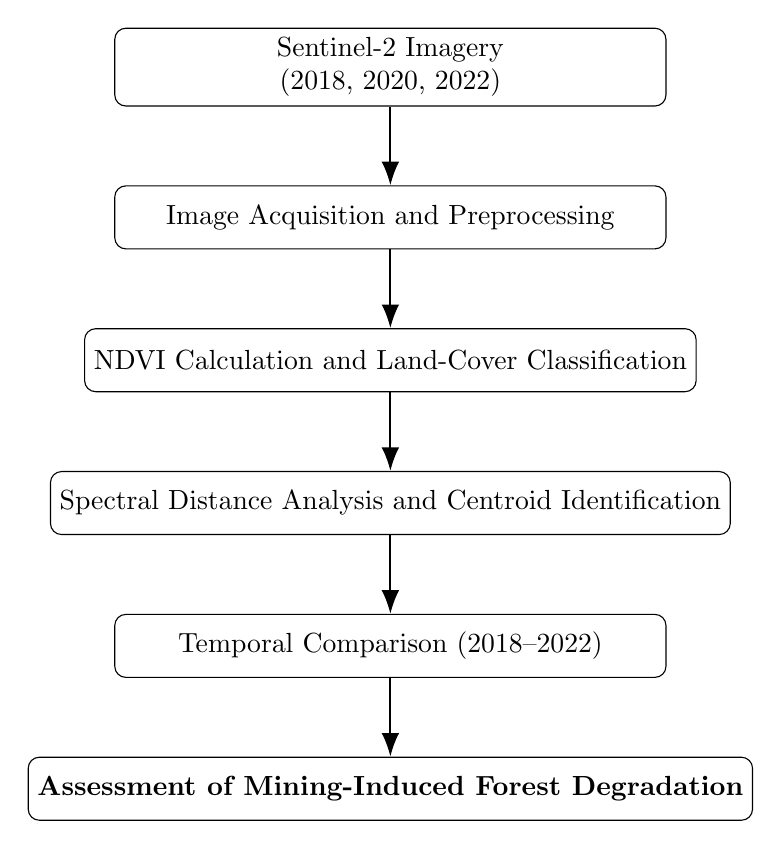
\begin{tikzpicture}[
node distance=1.0cm,
box/.style={
rectangle,
draw=black,
rounded corners,
minimum width=7cm,
minimum height=0.8cm,
align=center
},
arrow/.style={
-{Latex[length=3mm]},
thick
}
]

\node (a) [box] {Sentinel-2 Imagery\\(2018, 2020, 2022)};

\node (b) [box, below=of a]
{Image Acquisition and Preprocessing};

\node (c) [box, below=of b]
{NDVI Calculation and Land-Cover Classification};

\node (d) [box, below=of c]
{Spectral Distance Analysis and Centroid Identification};

\node (e) [box, below=of d]
{Temporal Comparison (2018--2022)};

\node (f) [box, below=of e]
{\textbf{Assessment of Mining-Induced Forest Degradation}};

\draw [arrow] (a) -- (b);
\draw [arrow] (b) -- (c);
\draw [arrow] (c) -- (d);
\draw [arrow] (d) -- (e);
\draw [arrow] (e) -- (f);

\end{tikzpicture}

\caption{Methodological framework used for assessing mining-induced forest degradation in the Pra River Basin.}
\label{fig:method_framework}

\end{figure}


The methodological framework consisted of four main stages:

\begin{itemize}
\item Image acquisition and preprocessing
\item NDVI calculation and land-cover classification
\item Spectral distance analysis
\item Temporal assessment of forest degradation
\end{itemize}


\section{Data Sources}

This study utilized Sentinel-2 Level-2A multispectral satellite imagery acquired from the Copernicus Open Access Hub to assess changes in vegetation condition within the Pra River Basin.

Three image dates were selected to represent the baseline, intermediate, and recent stages of environmental change:

\begin{itemize}
\item 12 January 2018
\item 2 January 2020
\item 26 January 2022
\end{itemize}

The images were selected during the dry season in order to minimize seasonal differences in vegetation condition. Only scenes with less than 10\% cloud cover were used.

Sentinel-2 imagery was chosen due to its high spatial resolution (10 m) and availability of spectral bands suitable for vegetation analysis, particularly in the red and near-infrared regions \citep{drusch2012sentinel}. These bands are essential for calculating vegetation indices such as the Normalized Difference Vegetation Index (NDVI).

The analysis focused on four Sentinel-2 bands. The spectral bands used in the analysis are summarized in Table~\ref{tab:bands}.

\begin{table}[H]
\centering
\caption{Sentinel-2 bands used in the analysis}
\label{tab:bands}

\begin{tabular}{lll}
\toprule
Band & Description & Spatial Resolution \\
\midrule
Band 2 & Blue & 10 m \\
Band 3 & Green & 10 m \\
Band 4 & Red & 10 m \\
Band 8 & Near Infrared (NIR) & 10 m \\
\bottomrule
\end{tabular}

\end{table}
The red and near-infrared bands were used for NDVI calculation, while all four bands were used in the spectral distance and fuzzy classification analysis.

\section{Image Preprocessing}

Prior to analysis, all Sentinel-2 images were preprocessed to ensure consistency across years. The preprocessing procedure included:

\begin{itemize}
\item Reprojection of all bands to a common coordinate reference system
\item Spatial alignment of the images
\item Clipping of the imagery to the approximate extent of the Pra River Basin
\item Removal of cloud-contaminated areas where necessary
\end{itemize}

All images were processed in the WGS 84 / UTM Zone 30N coordinate system. Using a common coordinate system ensured that spatial comparisons between 2018, 2020, and 2022 were accurate.

After preprocessing, true-colour and false-colour composites were created for visual interpretation.

The true-colour composite used the red, green, and blue bands:

\begin{itemize}
\item Red = Band 4
\item Green = Band 3
\item Blue = Band 2
\end{itemize}

The false-colour composite used the near-infrared, red, and green bands:

\begin{itemize}
\item Red = Band 8 (NIR)
\item Green = Band 4
\item Blue = Band 3
\end{itemize}

The false-colour composite was particularly useful because healthy vegetation appears in bright red tones, making areas of vegetation loss and mining disturbance easier to identify.


\section{NDVI Calculation}

The Normalized Difference Vegetation Index (NDVI) was used to quantify vegetation condition within the study area. NDVI was calculated separately for 2018, 2020, and 2022 using the red and near-infrared bands of Sentinel-2 imagery.

\begin{equation}
NDVI = \frac{NIR - Red}{NIR + Red}
\end{equation}

where $NIR$ represents near-infrared reflectance from Sentinel-2 Band 8, and $Red$ represents red reflectance from Sentinel-2 Band 4.

NDVI values range from -1 to +1. High NDVI values indicate dense and healthy vegetation, whereas low NDVI values indicate bare soil, water, mining surfaces, or degraded land.

NDVI maps were generated for each year in order to evaluate changes in vegetation condition over time. These maps provided the basis for identifying vegetation loss, disturbed vegetation, and potential mining-related land-cover change within the Pra River Basin.
The NDVI approach has been widely applied in vegetation monitoring and environmental assessment \citep{tucker1979ndvi}.


\section{NDVI-Based Classification and Change Detection}

A rule-based classification procedure was developed to distinguish major land-cover types within the Pra River Basin. The classification was based on NDVI threshold values, which were defined using typical vegetation characteristics in tropical environments and refined through visual comparison with true-colour and false-colour composite images.

The classification scheme is summarized in Table~\ref{tab:ndvi_classes}.
The threshold values were based on commonly reported NDVI ranges for tropical vegetation and non-vegetated surfaces and were refined through visual interpretation of the Sentinel-2 true-colour and false-colour composites.

\begin{table}[H]
\centering
\caption{NDVI-based land-cover and change-detection classification scheme}
\label{tab:ndvi_classes}

\begin{tabular}{lll}
\toprule
Class & NDVI Range / Condition & Interpretation \\
\midrule
1 & NDVI < 0.05 & Water Bodies \\
2 & NDVI < 0.30 (2022) and NDVI > 0.45 (2018) & Mining disturbance \\
3 & NDVI $\geq$ 0.40 & Healthy Vegetation \\
4 & 0.25 $\leq$ NDVI < 0.40 & Disturbed Vegetation \\
5 & 0.05 $\leq$ NDVI < 0.25 & Bare Soil \\
\bottomrule
\end{tabular}

\end{table}

Mining-related disturbance was identified using a change-based NDVI approach. Pixels that exhibited high NDVI values in 2018 (NDVI > 0.45), indicating healthy vegetation, and low NDVI values in 2022 (NDVI < 0.30), indicating vegetation removal or severe disturbance, were classified as areas of likely mining-related vegetation loss.

This classification represents a change-detection indicator derived from NDVI differences between 2018 and 2022, rather than a direct land-cover class. It is based on the assumption that substantial vegetation loss within the study area is strongly associated with mining-related land disturbance. This approach also improves discrimination between true vegetation loss and naturally occurring bare surfaces or other stable non-vegetated land-cover types.



\section{Spectral Distance Analysis}

Although NDVI is effective for identifying major differences between vegetated and non-vegetated surfaces, it may not detect more subtle changes in forest condition. For this reason, spectral distance analysis was applied to complement the NDVI-based classification.

The analysis used four Sentinel-2 spectral bands (blue, green, red, and near-infrared), which were combined into a multi-band spectral stack for each year. To reduce computational demand, the spectral data were aggregated from 10 m to 100 m spatial resolution.

Spectral centroids representing dominant land-cover classes were identified from the 2018 dataset and used as reference signatures for subsequent years.

The spectral distance between each pixel and the reference centroid was calculated using Euclidean distance:

\begin{equation}
D = \sqrt{(B - B_c)^2 + (G - G_c)^2 + (R - R_c)^2 + (NIR - NIR_c)^2}
\end{equation}

where $D$ represents the spectral distance, $B$, $G$, $R$, and $NIR$ represent the observed pixel reflectance values, and $B_c$, $G_c$, $R_c$, and $NIR_c$ represent the centroid values of the reference class.

Spectral distance analysis has been widely used in remote sensing studies to evaluate landscape change and vegetation disturbance \citep{richards2013remote}.

Lower spectral distance values indicate greater similarity to the reference condition, while higher values indicate greater spectral divergence from the baseline forest condition and therefore greater forest degradation.

This approach allows the detection of gradual changes in forest condition that may not be captured by NDVI alone.


\section{Fuzzy Classification Procedure}

A fuzzy classification approach was applied to identify spectral centroids and quantify the similarity of each pixel to different land-cover classes. Unlike traditional classification methods that assign each pixel to a single class, fuzzy classification allows pixels to have partial membership across multiple classes, providing a more realistic representation of heterogeneous landscapes.

The fuzzy classification procedure consisted of the following steps:

\begin{itemize}
\item The four-band spectral stack from 2018 (blue, green, red, and near-infrared) was used as the baseline dataset.
\item K-means clustering was applied to divide the image into three major spectral classes.
\item Three clusters were selected because the primary objective was to distinguish healthy vegetation, mining-related surfaces, and intermediate transitional conditions within the landscape.
\item The resulting cluster centroids were interpreted based on their spectral characteristics.
\item The centroid with the highest Red/NIR ratio was identified as the mining class.
\item The centroid with the highest NDVI value was identified as the healthy vegetation class.
\item The same 2018 centroids were applied to the 2020 and 2022 imagery.
\end{itemize}

Applying the same centroids across all years ensured that spectral changes could be compared consistently over time.

Fuzzy membership values were then calculated for each pixel to determine the degree to which it belonged to each class. Pixels with higher membership to the forest class were considered more similar to healthy vegetation, while pixels with lower membership and greater spectral distance were interpreted as degraded.

This approach allows for the detection of gradual transitions between land-cover types and provides a more detailed assessment of mining-induced forest degradation.



\section{Temporal Analysis}

Changes in vegetation condition and forest degradation were assessed by comparing NDVI values, land-cover classifications, and spectral distance results across the three time periods (2018, 2020, and 2022).

This temporal comparison enabled the identification of trends in vegetation loss, forest degradation, and mining-related disturbance within the study area \citep{lu2004change,singh1989review}.



\chapter{Results}

This chapter presents the results of the multi-temporal remote sensing analysis conducted for the Pra River Basin. The results are organized into NDVI time-series analysis, NDVI change detection, land-cover classification, spatial distribution of mining activity, and spectral distance analysis of mining and forest condition.

\section{NDVI Time-Series Analysis}

The NDVI maps for 2018, 2020, and 2022 show a progressive decline in vegetation condition and vegetation loss within the Pra River Basin.

In 2018, most parts of the basin exhibited relatively high NDVI values, indicating the presence of dense and healthy vegetation. High positive NDVI values dominated the central and western portions of the study area.

By 2020, localized areas of lower NDVI had begun to appear, particularly within the central portion of the basin and in areas associated with mining activity. These patterns indicate the early stages of vegetation loss within the study area.

The 2022 NDVI map shows a much larger extent of reduced NDVI values. Areas of low NDVI became more widespread across the basin, particularly within the central degraded zone and surrounding landscapes. Several areas that previously exhibited high NDVI in 2018 had transitioned to values characteristic of disturbed vegetation, bare soil, or or mining-related surfaces.

The largest change in vegetation condition and vegetation loss occurred between 2020 and 2022, as shown in Figure~\ref{fig:ndvi_timeseries}.

\begin{figure}[H] \centering \includegraphics[width=0.9\textwidth]{maps/ndvi_timeseries.png} \caption{NDVI maps showing vegetation condition in 2018, 2020, and 2022.} \label{fig:ndvi_timeseries} \end{figure}


\section{NDVI Change Detection and Distribution}

The NDVI change map for 2018--2022 illustrates the spatial distribution of vegetation condition change within the Pra River Basin. Areas classified as vegetation decrease are shown in orange and represent locations where NDVI values declined between 2018 and 2022, indicating a reduction in vegetation condition or cover. Areas classified as vegetation increase are shown in blue and represent locations where vegetation greenness improved during the study period. Grey areas indicate little or no detectable change in vegetation condition.

The map reveals that vegetation decrease was considerably more widespread than vegetation recovery across the basin. Areas classified as vegetation decrease occur throughout the study area, with notable concentrations in mining-affected landscapes. In contrast, areas of vegetation increase are limited and occur only in small, scattered patches. The predominance of vegetation decline suggests that land disturbance processes had a greater influence on vegetation condition change than natural regeneration during the study period.

The accompanying NDVI change distribution chart shows that 69.1\% of the study area experienced little or no detectable change in vegetation condition between 2018 and 2022. However, 29.3\% of the basin was classified as vegetation decrease, while only 1.7\% was classified as vegetation increase. These results indicate that vegetation loss substantially exceeded vegetation recovery across the basin.

Overall, the combined map and bar chart demonstrate that although most of the Pra River Basin remained relatively stable, vegetation decline was the dominant pattern during the study period. The spatial concentration of vegetation loss within mining-affected landscapes suggests that mining activities contributed to localized vegetation degradation and land-cover disturbance within the basin.

\begin{figure}[H]
\centering
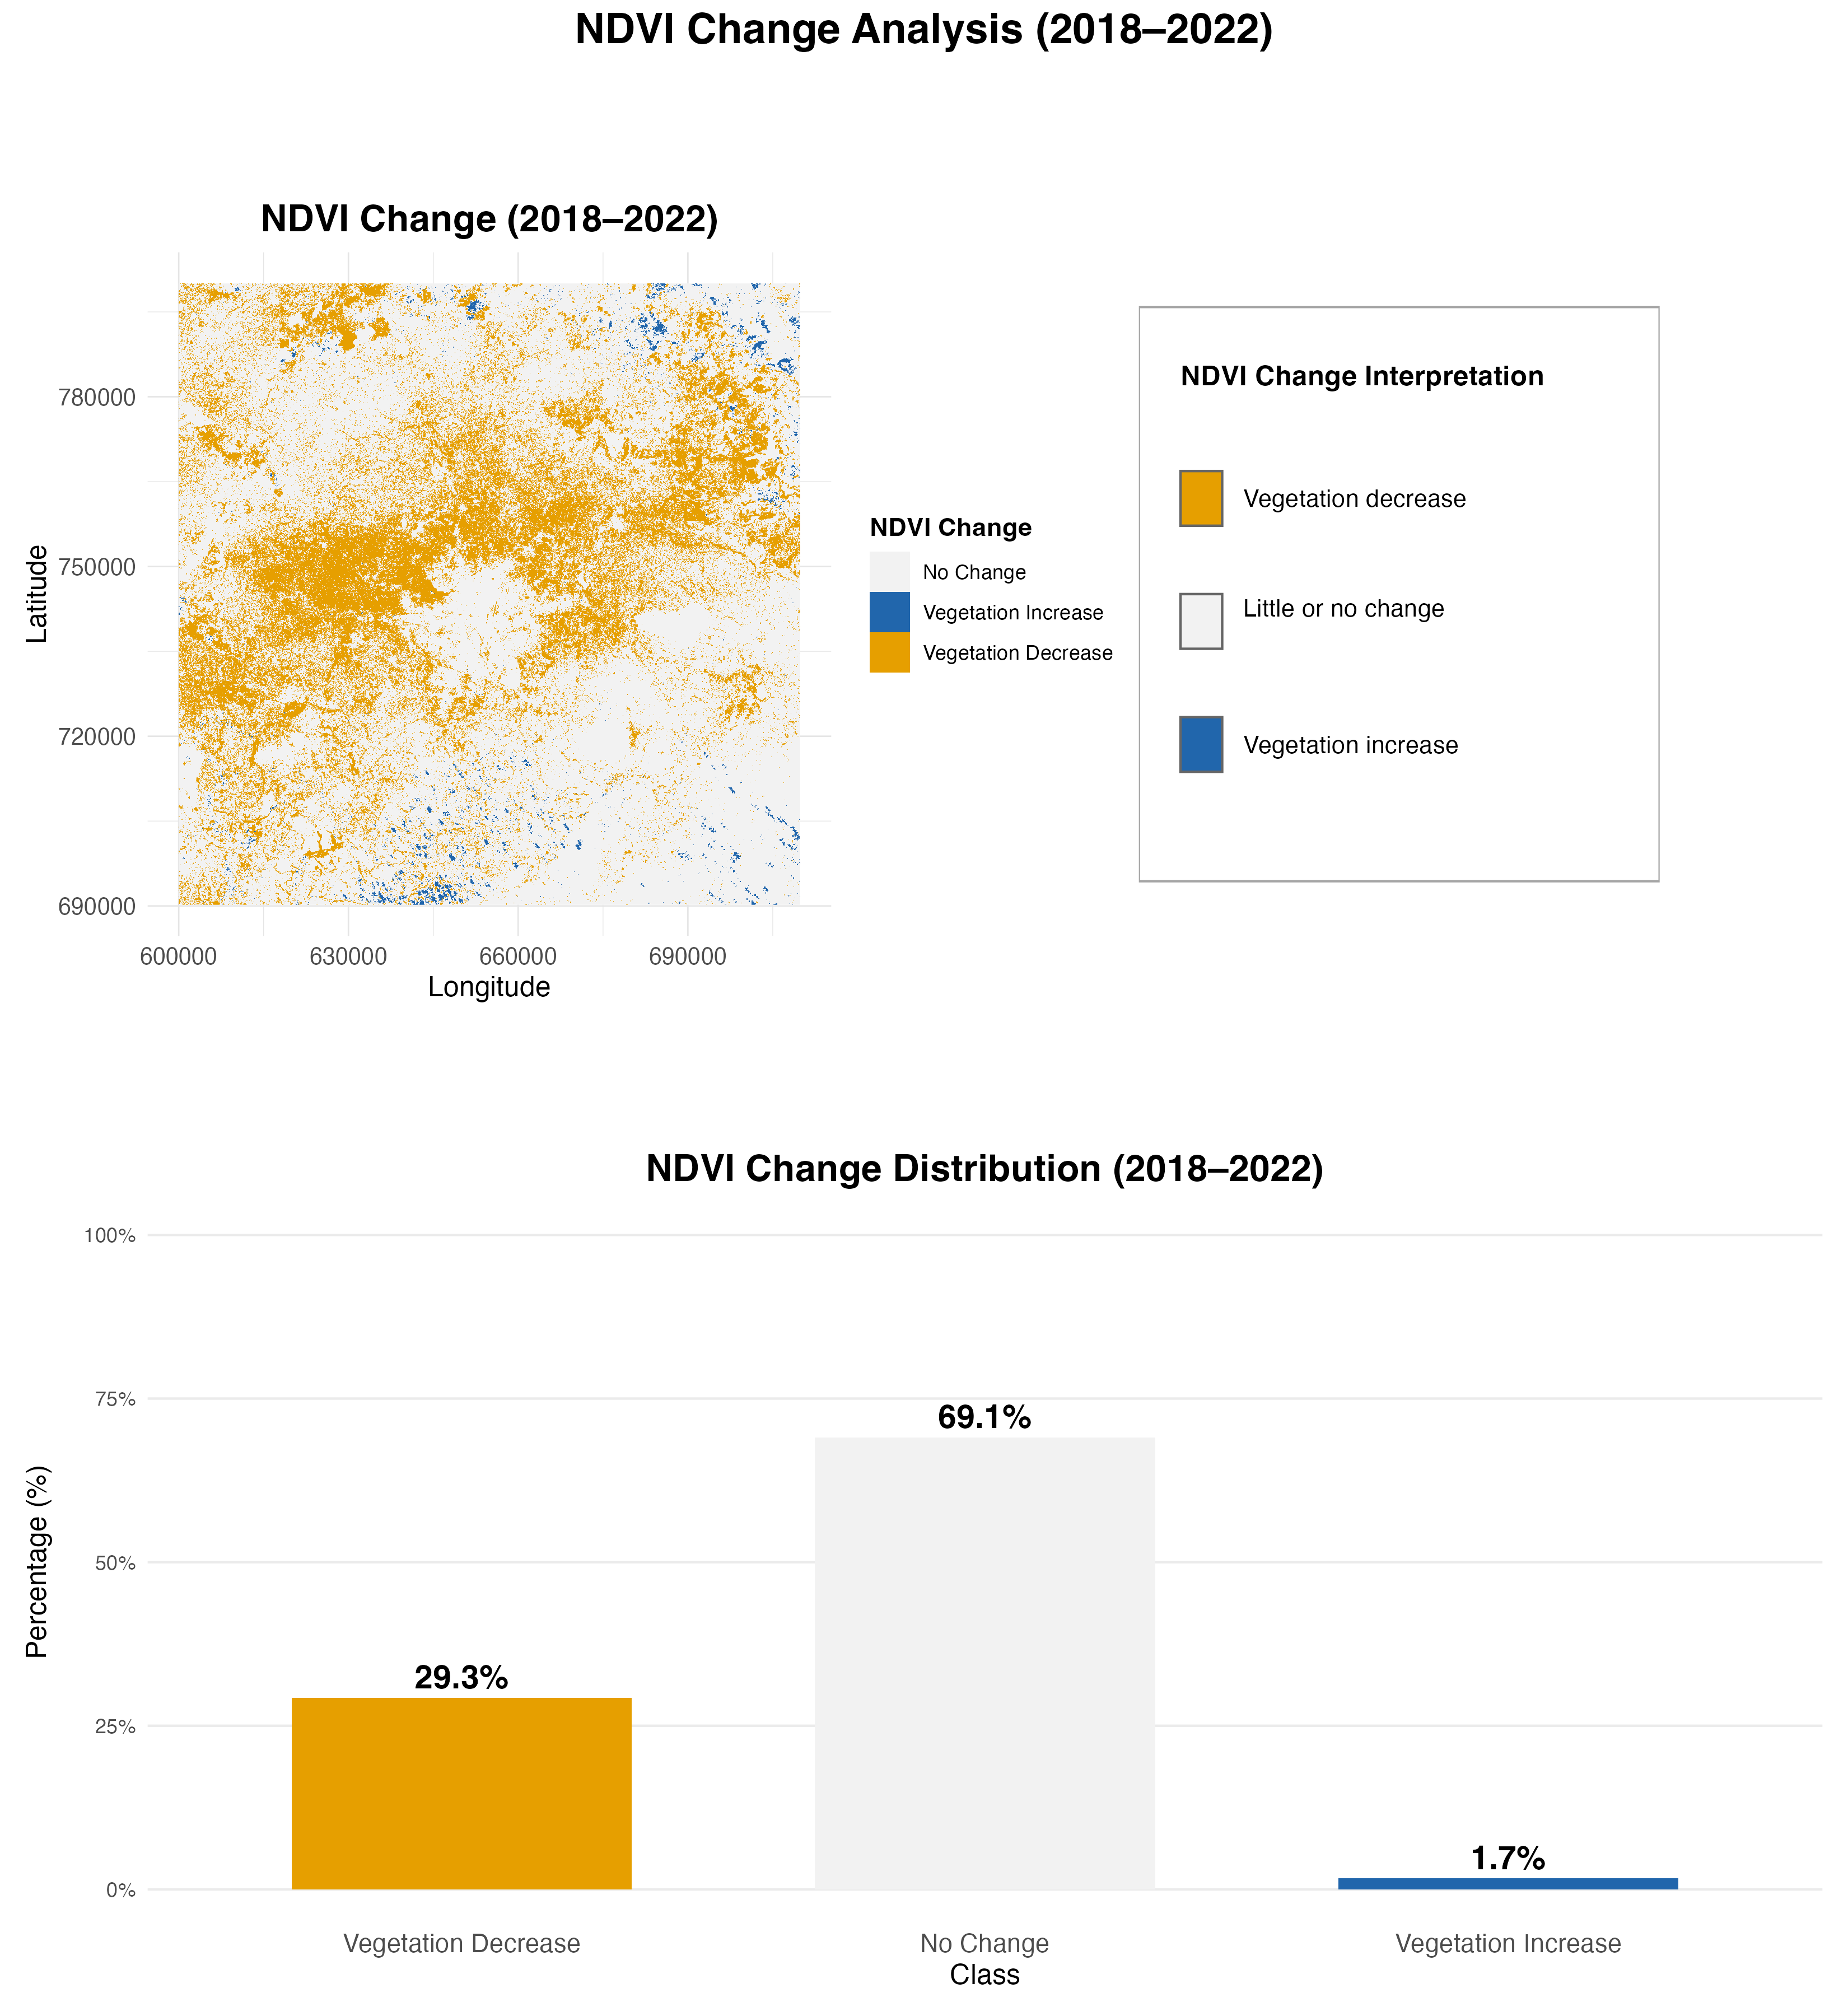
\includegraphics[width=\textwidth,height=0.82\textheight,keepaspectratio]{maps/ndvi_change_map_and_bar_chart.png}
\caption{NDVI change map and NDVI change distribution in the Pra River Basin between 2018 and 2022.}
\label{fig:ndvi_change_combined}
\end{figure}



\section{Land-Cover Classification}

The NDVI-based classification distinguished five land-cover classes within the Pra River Basin: water bodies, mining disturbance, healthy vegetation, disturbed vegetation, and bare soil.

Disturbed vegetation represented the dominant land-cover class in 2022, followed by healthy vegetation and bare soil. The prevalence of disturbed vegetation suggests that large portions of the basin have experienced varying degrees of landscape modification and ecological disturbance.

Disturbed vegetation was concentrated around mining disturbance areas and adjacent landscapes, suggesting that the effects of mining extend beyond the areas of direct excavation.

Mining disturbance pixels were concentrated mainly within the central and southern portions of the study area. Many of these pixels occurred in locations that had exhibited relatively high NDVI values in 2018, indicating recent vegetation loss consistent with mining-related land disturbance.

Bare soil areas were also identified around these zones, representing areas where vegetation had been removed but where no active vegetation recovery was observed.

The spatial distribution of classified land-cover types is shown in Figure~\ref{fig:classification_2022}.


\begin{figure}[H] \centering 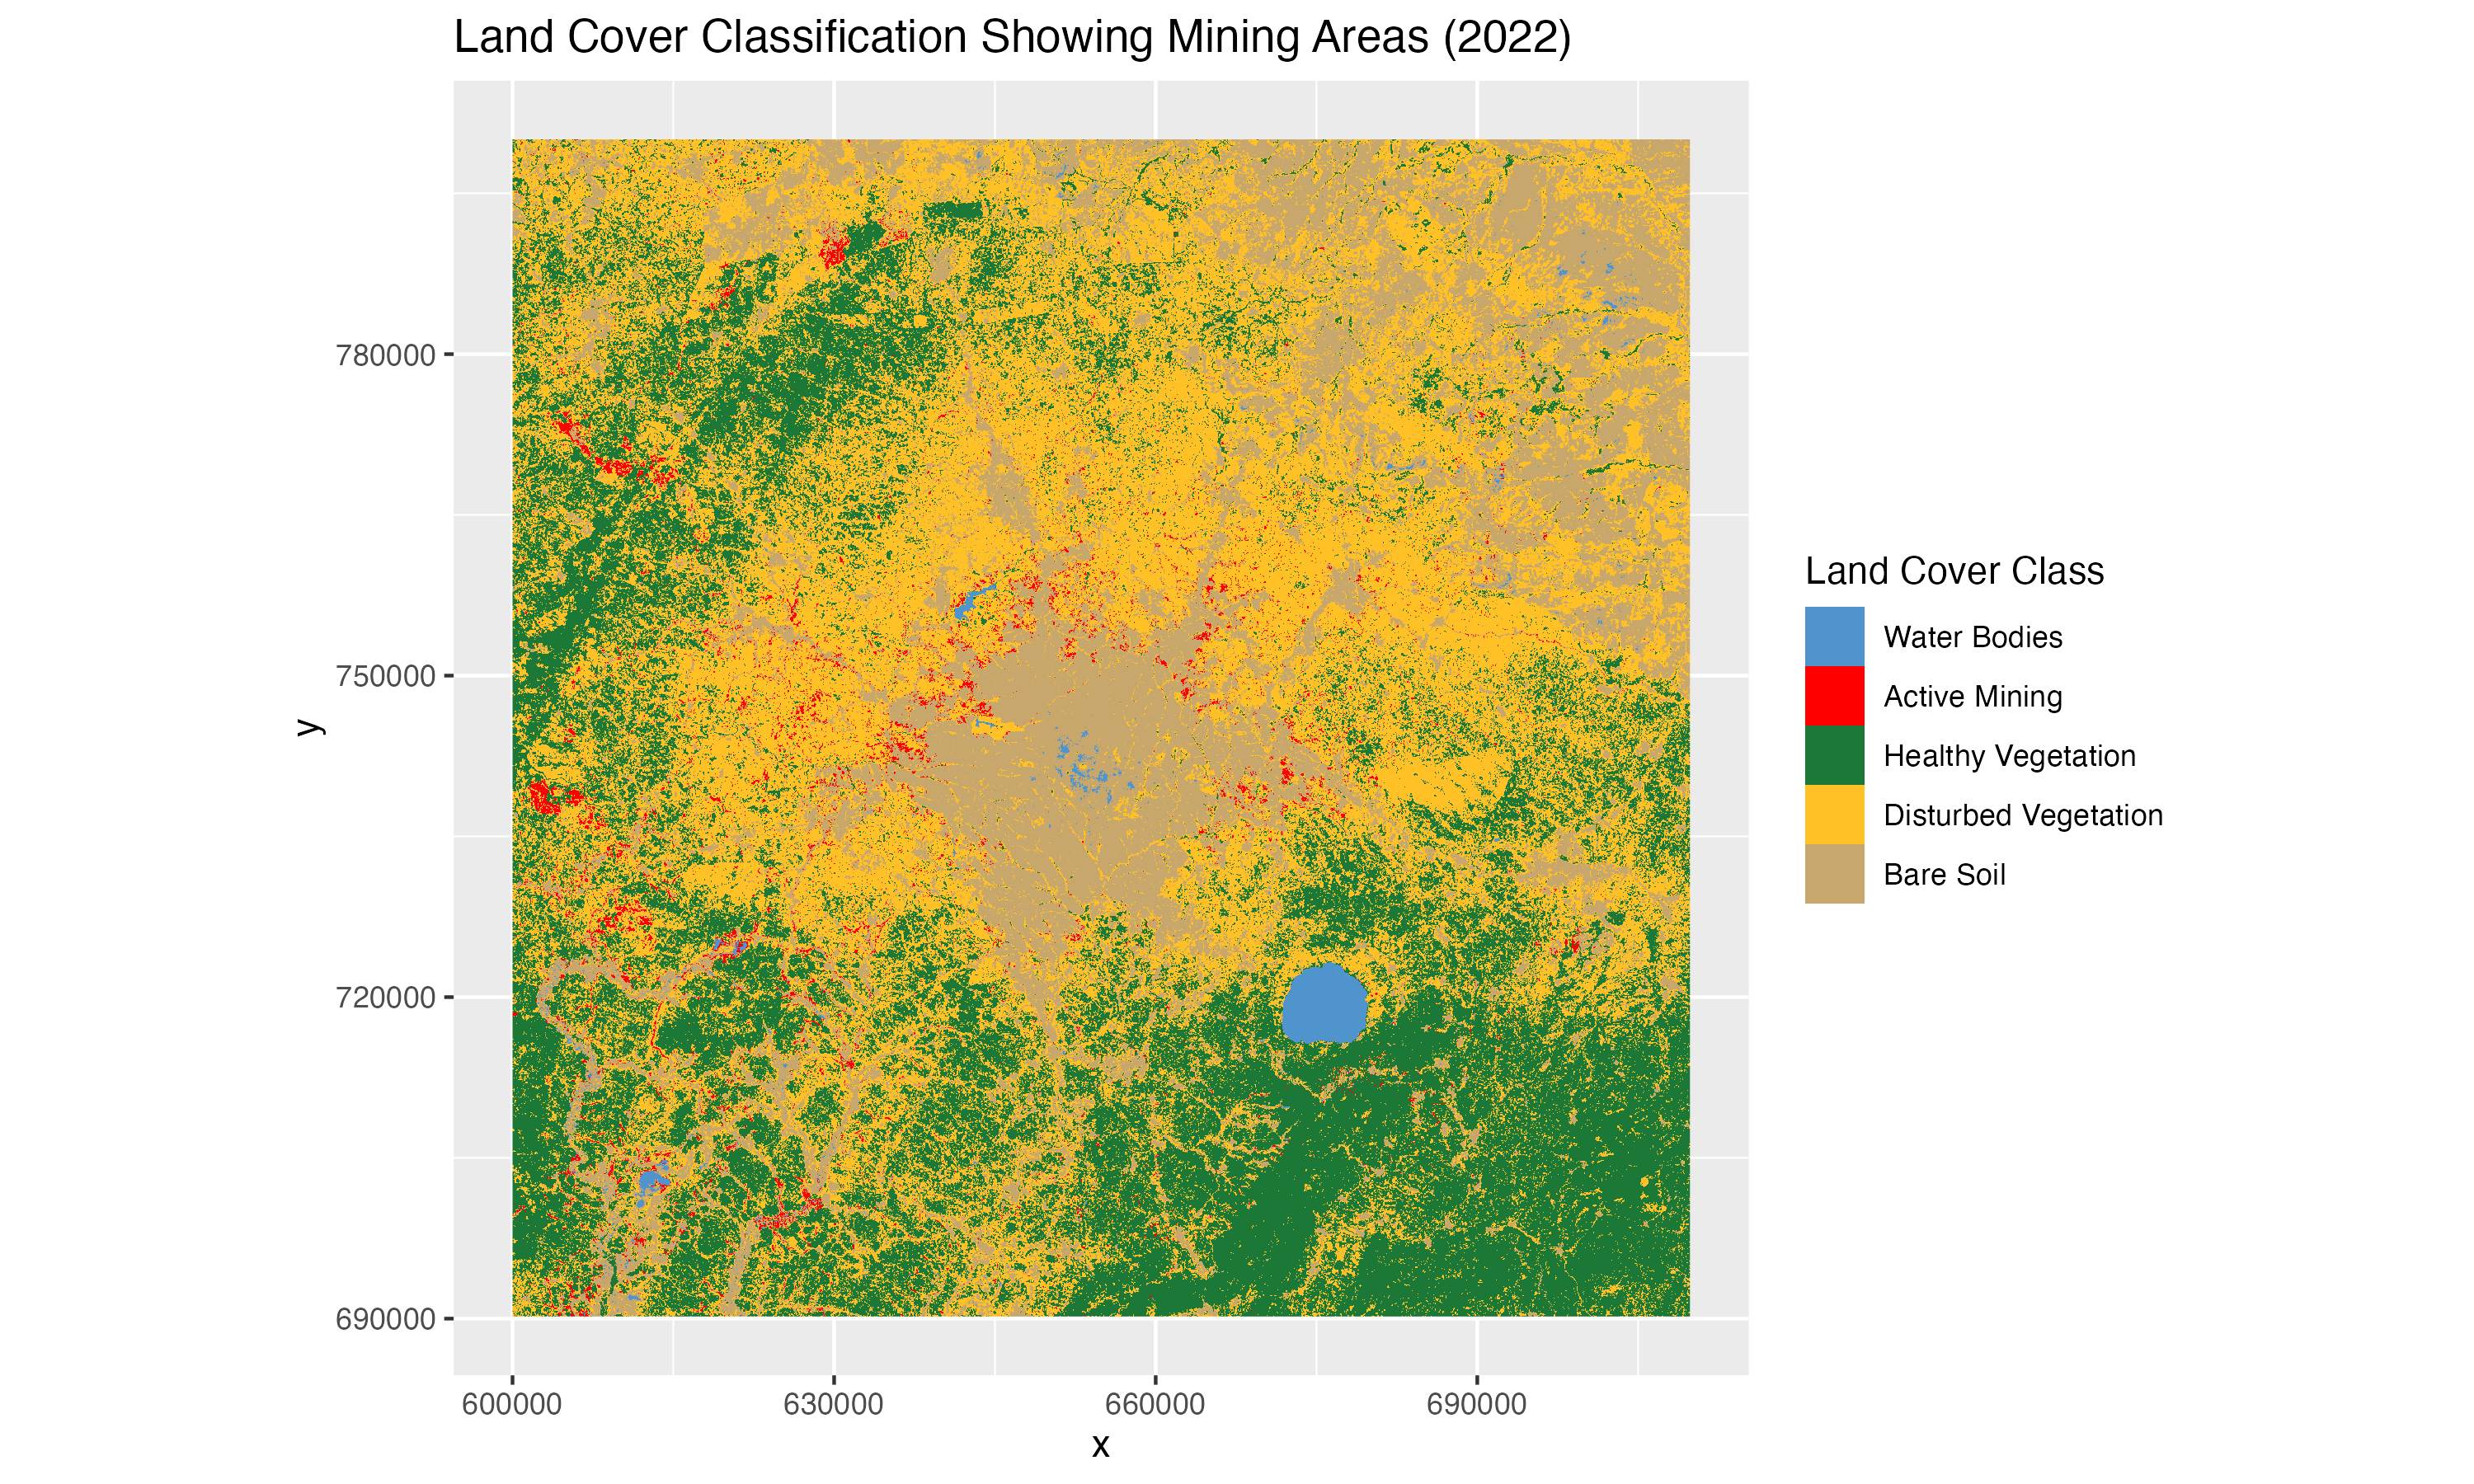
\includegraphics[width=0.85\textwidth,height=0.55\textheight,keepaspectratio]{maps/vegetation_mining_2022.png} \caption{NDVI-based land-cover classification showing mining disturbance areas in 2022.} \label{fig:classification_2022} \end{figure}


\subsection{Land Cover Classification and Distribution (2022)}

The land cover classification map for 2022 reveals a highly heterogeneous landscape within the Pra River Basin. Disturbed vegetation represents the largest land cover class, accounting for 43.1\% of the study area. This is followed by healthy vegetation, which covers 31.5\% of the basin. Bare soil constitutes 21.4\%, while mining disturbance and water bodies occupy relatively small proportions of 3.2\% and 0.9\%, respectively.

The dominance of disturbed vegetation and bare soil indicates that more than half of the basin (64.5\%) is characterised by modified or degraded land cover conditions. In contrast, intact or healthy vegetation covers less than one-third of the study area, suggesting significant landscape fragmentation.

Although mining disturbance occupies a relatively small spatial extent, its presence is concentrated in specific zones and is likely to contribute disproportionately to surrounding vegetation disturbance. This is supported by the NDVI change analysis, which also indicates widespread vegetation decline across the basin.

Overall, the land cover distribution highlights a landscape under considerable anthropogenic pressure, where disturbed and transitional land cover types dominate over stable vegetated conditions.

The spatial distribution of classified land-cover types is shown in Figure~\ref{fig:landcover_distribution_2022}.

\begin{figure}[H]
    \centering
    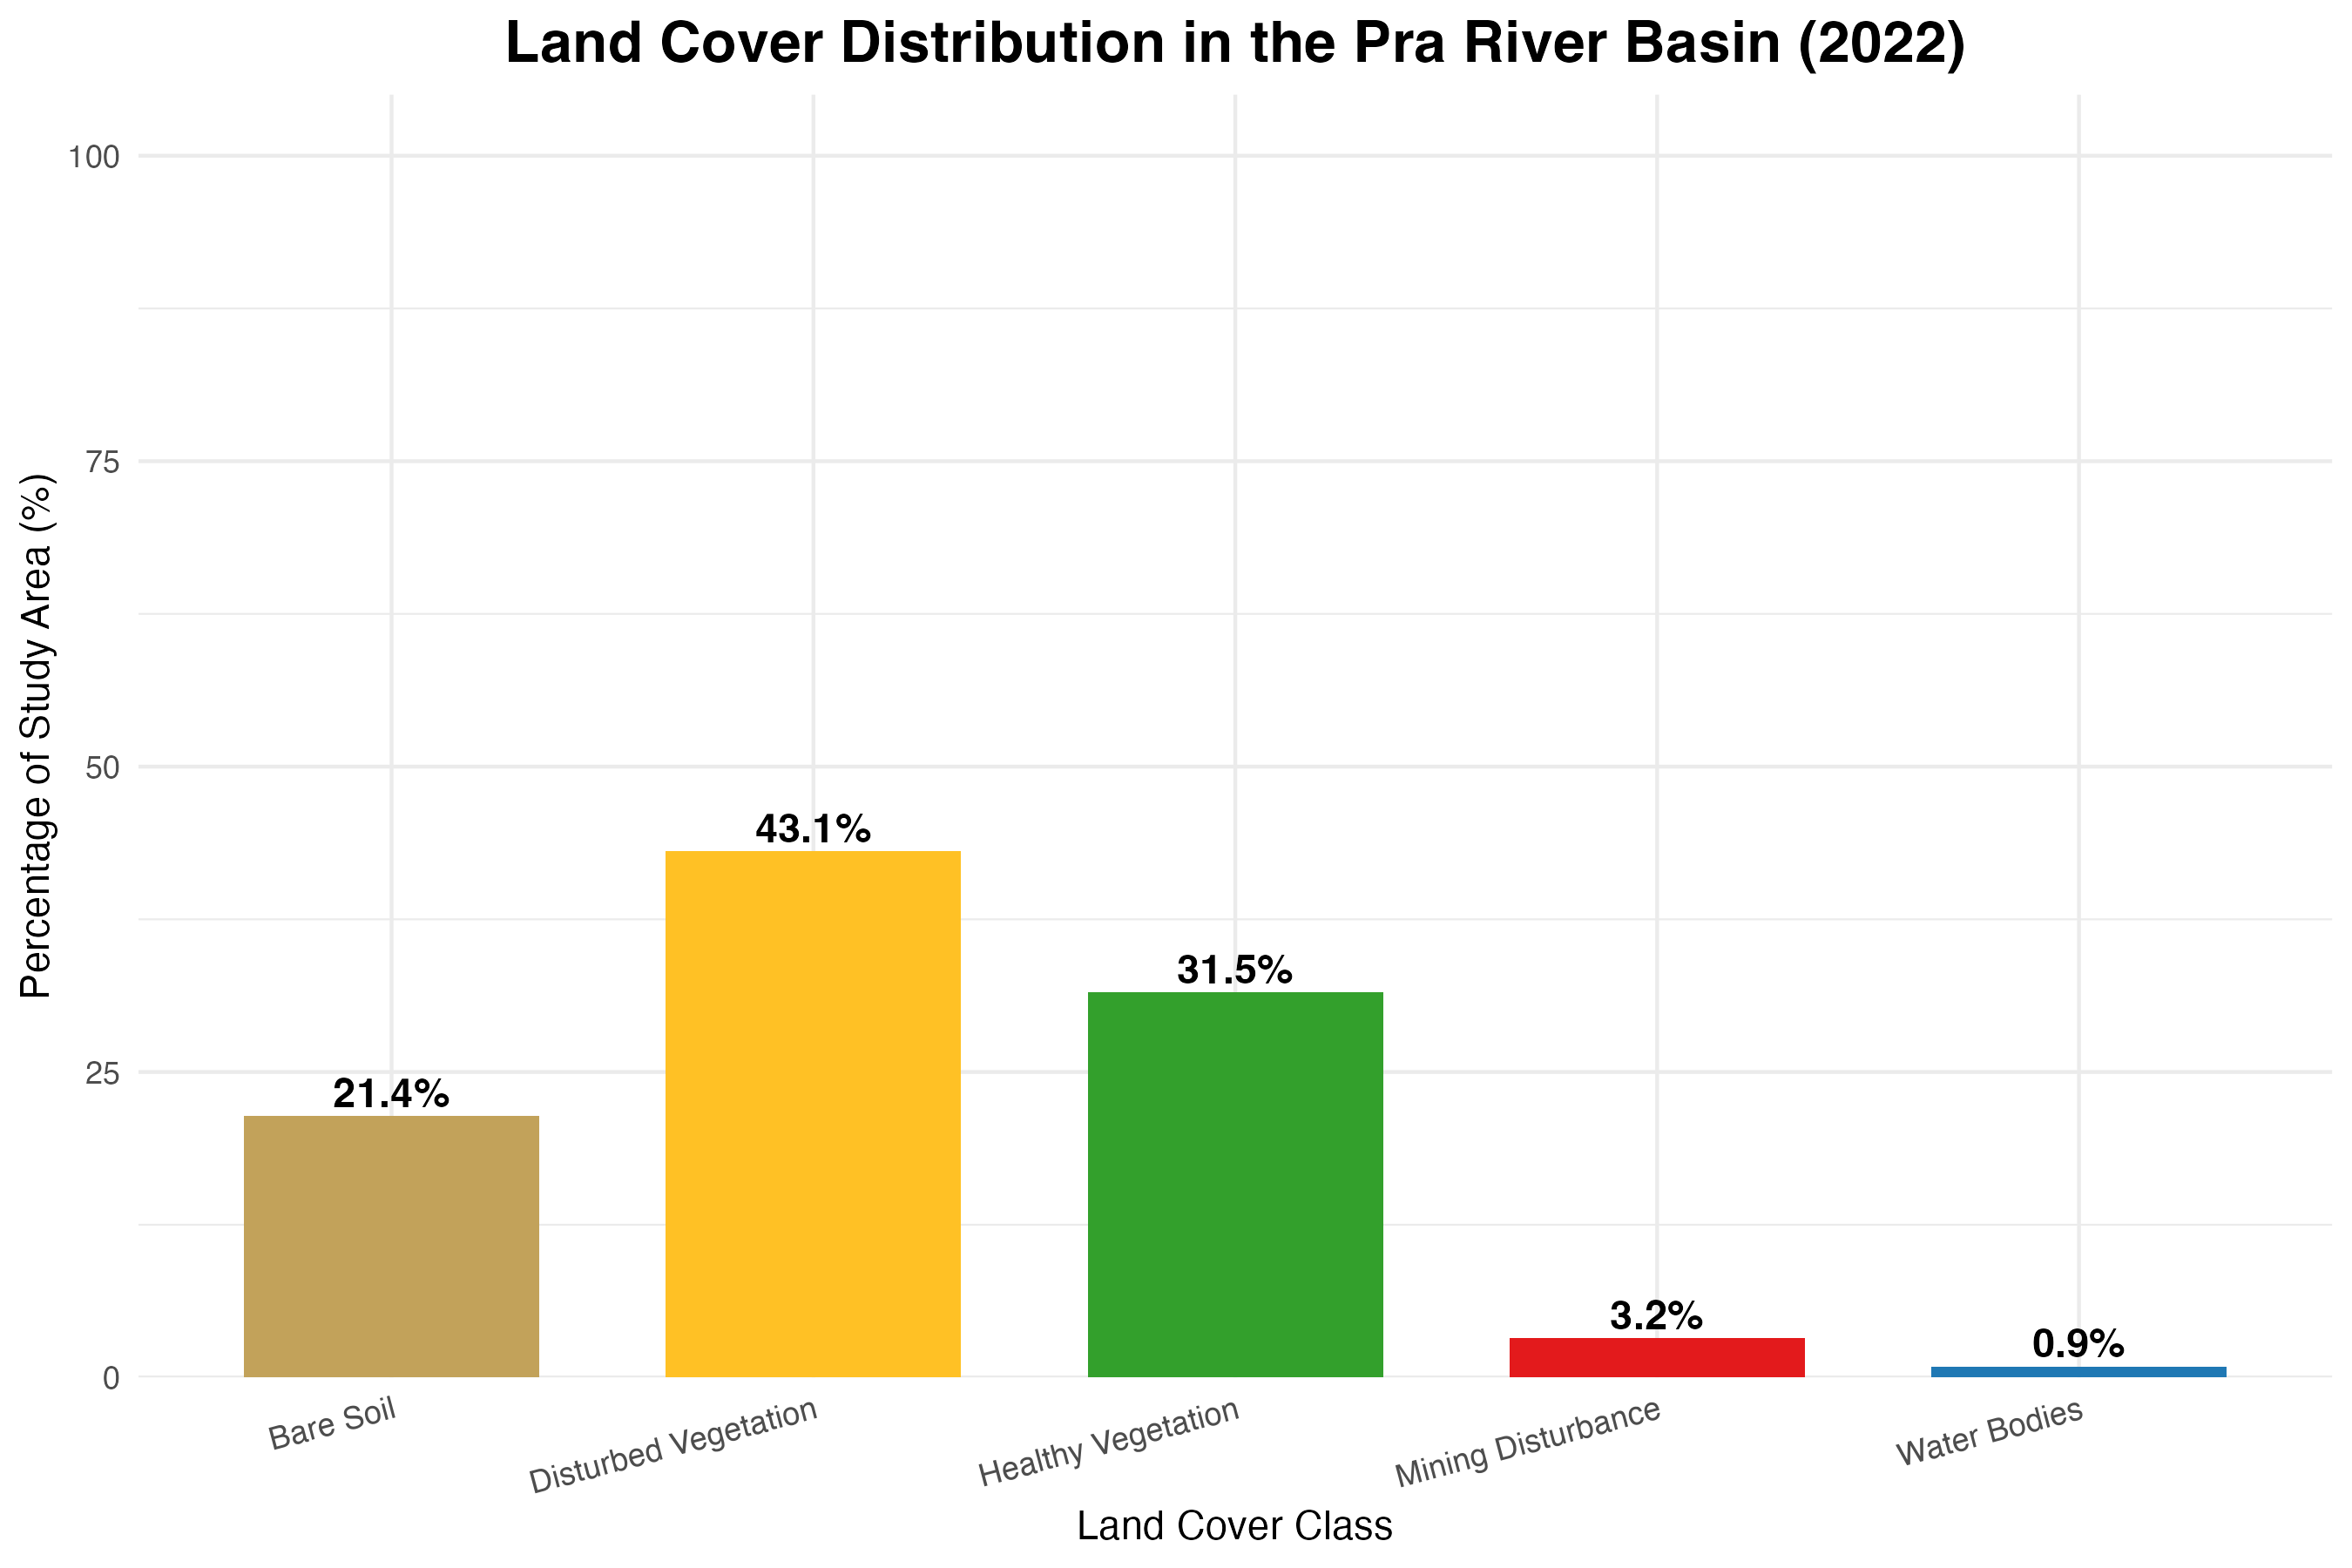
\includegraphics[width=0.85\textwidth,height=0.55\textheight,keepaspectratio]{maps/landcover_distribution_2022.png}
    \caption{Land-cover distribution in the Pra River Basin in 2022.}
    \label{fig:landcover_distribution_2022}
\end{figure}

\section{Spatial Distribution of Mining Disturbance}

The mining disturbance map shows that mining disturbance sites are concentrated within specific mining-influenced areas of the basin.

Mining disturbance is not evenly distributed across the study area but is instead clustered within several major mining zones, particularly in the central portion of the basin.

Several major mining clusters are visible in the central portion of the basin, while smaller mining disturbance areas are also present in the northern and southern parts of the study area.

The concentration of mining disturbance within specific mining-influenced zones suggests that mining activity may contribute not only to forest degradation but also to broader environmental disturbance across the basin.

When considered alongside the NDVI change and land-cover classification results, a clear spatial relationship emerges between mining disturbance and vegetation disturbance. Areas characterised by mining disturbance, disturbed vegetation, and bare soil frequently correspond with locations exhibiting vegetation decline, suggesting that land-cover modification is an important driver of the observed degradation patterns within the Pra River Basin.

The spatial distribution of mining disturbance is presented in Figure~\ref{fig:mining_distribution}.

\begin{figure}[H] \centering \includegraphics[width=0.82\textwidth,height=0.55\textheight,keepaspectratio]{maps/mining_distribution_map_2022.png} \caption{Spatial distribution of mining disturbance in the Pra River Basin in 2022.} \label{fig:mining_distribution} \end{figure}



\section{Spectral Analysis of Mining Disturbance}

The spectral distance analysis shows that the spectral properties of the landscape became progressively more similar to the mining centroid between 2018 and 2022. The change in mining disturbance spectral condition is shown in Figure~\ref{fig:mining_spectral}.

In 2018, most pixels exhibited relatively large distances from the mining centroid, indicating that mining disturbance surfaces occupied only a limited proportion of the study area. By 2020, the distribution shifted slightly toward lower distances, suggesting an increase in mining disturbance-related surfaces. The strongest shift occurred in 2022, when a larger proportion of pixels exhibited low spectral distance to the mining centroid. This indicates that mining disturbance expanded substantially during the study period.

The density distribution shown in Figure~\ref{fig:mining_spectral} demonstrates this progressive temporal shift toward lower spectral distances, indicating increasing similarity of landscape conditions to the mining reference signature over time.

The scatter plot further illustrates the distribution of landscape pixels within spectral space using red and near-infrared reflectance values. The mining centroid, shown as the red diamond, represents the reference mining disturbance spectral signature derived from the 2018 dataset. Pixels located closer to this centroid exhibit greater spectral similarity to mining disturbance surfaces, whereas pixels located farther away represent less disturbed land-cover conditions. The broader spread observed in later years suggests increasing spectral heterogeneity associated with mining disturbance expansion.

\begin{figure}[H] \centering 
\includegraphics[width=\textwidth,height=0.5\textheight,keepaspectratio]{maps/mining_spectral_analysis.png} \caption{Spectral distance of landscape pixels to the mining centroid between 2018 and 2022.} \label{fig:mining_spectral} \end{figure}

\section{Spectral Analysis of Forest Condition}

The spectral analysis of forest condition reveals an opposite trend to that observed for mining disturbance. The change in forest spectral condition is shown in Figure~\ref{fig:forest_spectral}.

In 2018, most pixels exhibited low spectral distance from the forest centroid, indicating that the landscape retained characteristics similar to healthy forest conditions. By 2020, the distribution shifted slightly toward higher distances, suggesting the early stages of forest degradation. The most pronounced shift occurred in 2022, where a larger proportion of pixels exhibited high spectral distance from the forest centroid, indicating increasing divergence from the original forest condition.

The density distribution shown in Figure~\ref{fig:forest_spectral} demonstrates this progressive temporal shift toward larger spectral distances, indicating that forest areas became increasingly dissimilar to the 2018 reference condition over time.

The scatter plot further illustrates the distribution of landscape pixels relative to the healthy forest centroid represented by the green diamond. Pixels located closer to the centroid retain spectral characteristics more similar to healthy vegetation, while increasing distance indicates greater divergence from the reference forest condition. The wider spread observed in 2022 suggests progressive degradation and increasing variation in vegetation condition across the landscape.

\begin{figure}[H] \centering 
\includegraphics[width=\textwidth,height=0.5\textheight,keepaspectratio]{maps/forest_spectral_analysis.png} \caption{Spectral distance of landscape pixels to the forest centroid between 2018 and 2022.} \label{fig:forest_spectral} \end{figure}

\section{Summary of Results}

The results demonstrate that vegetation condition declined substantially between 2018 and 2022 within the Pra River Basin. NDVI analysis revealed widespread reductions in vegetation condition, particularly in areas affected by mining disturbance.

Mining disturbance expanded considerably during the study period and was concentrated within specific mining-influenced areas of the basin. At the same time, spectral distance analysis showed that remaining forest areas became progressively less similar to the 2018 healthy forest reference condition.

These findings indicate that mining disturbance contributed not only to direct vegetation removal but also to broader forest degradation across the surrounding landscape. The combined use of NDVI and spectral distance analysis therefore provided complementary evidence of both land-cover change and gradual ecological deterioration within the study area.

\FloatBarrier

\chapter{Discussion}

This chapter discusses the findings of the study in relation to the research objectives and existing literature on mining-induced forest degradation and remote sensing analysis. The discussion focuses on the observed patterns of vegetation decline within the Pra River Basin, the spatial relationship between mining activity and forest degradation, and the effectiveness of integrating NDVI and spectral distance analysis for environmental monitoring. The implications of the findings for forest management and environmental sustainability are also considered.

\section{Vegetation Decline within the Pra River Basin}

The results of the NDVI time-series analysis revealed a progressive decline in vegetation condition across the Pra River Basin between 2018 and 2022. Areas that exhibited relatively high NDVI values in 2018 showed substantial reductions by 2022, indicating increasing vegetation disturbance and vegetation loss over time \citep{asner2005selective,sonter2017mining,hilson2002environmental}

The largest decline in vegetation condition occurred between 2020 and 2022, suggesting that forest disturbance accelerated during the latter part of the study period. This pattern is consistent with reports of increasing artisanal and illegal mining activities in southern Ghana during recent years. The widespread reduction in NDVI values indicates that mining-related disturbance has likely contributed to vegetation loss and forest degradation within the basin.

The NDVI difference map further demonstrated that vegetation decrease was concentrated within mining-influenced landscapes. This spatial pattern reflects the concentration of mining disturbance within specific portions of the basin and the associated removal of vegetation in surrounding landscapes. As vegetation is removed for excavation and mining infrastructure, surrounding forest areas become increasingly fragmented and degraded.

The NDVI change distribution analysis showed that vegetation decrease accounted for a larger proportion of the study area than vegetation increase. Although most areas remained relatively stable, the proportion of vegetation decline indicates that mining-related disturbance represents a significant environmental concern within the basin.

This interpretation is further supported by the land-cover classification results, which showed that disturbed vegetation and bare soil together accounted for 64.5\% of the basin, substantially exceeding the area occupied by healthy vegetation. The predominance of disturbed land-cover types provides additional evidence of widespread landscape modification within the study area.

These findings support previous studies that identified mining as a major driver of forest degradation in tropical regions \citep{asner2005selective,sonter2017mining}. They are also consistent with studies conducted in Ghana and the Pra River Basin, which reported substantial vegetation loss and land-cover transformation associated with mining expansion \citep{awotwi2018pra,barenblitt2021ghana}.

\section{Spatial Relationship Between Mining Disturbance and Forest Degradation}

The spatial distribution of mining disturbance features showed that mining-related features were strongly clustered within several mining-influenced zones across the basin. This clustering pattern demonstrates the close relationship between mining-related land disturbance and riverine environments within the basin.

The mapped mining disturbance areas revealed that many sites were located within or adjacent to previously vegetated areas. Areas surrounding these clusters also exhibited lower NDVI values and greater spectral divergence from the healthy forest reference condition. This indicates that the environmental effects of mining disturbance extend beyond the immediate excavation sites.

The concentration of disturbed vegetation around mining disturbance areas suggests that mining is associated not only with direct vegetation removal but also with broader ecological degradation. Mining activities often expose surrounding vegetation to sediment deposition, soil instability, hydrological disruption, and increased human disturbance \citep{hilson2002environmental,sonter2017mining}. These processes may reduce vegetation health even where forest remains partially intact and may accelerate long-term ecological deterioration within tropical forest systems \citep{tarazona2020monitoring}.

The results therefore suggest that mining-related forest degradation is strongly associated with both direct and indirect mechanisms. Direct impacts involve the physical removal of vegetation, while indirect impacts involve gradual deterioration in forest condition surrounding mining disturbance zones.

This finding agrees with previous research indicating that mining frequently produces landscape-scale environmental effects that extend beyond active extraction areas \citep{hilson2002land,sonter2017mining}. Similar patterns have been documented in Ghana, where mining expansion has been associated with extensive vegetation loss and disturbance across broader landscapes rather than only within active mining sites \citep{barenblitt2021ghana,awotwi2018pra}.

\section{Interpretation of Spectral Distance Analysis}

The spectral distance analysis provided additional insight into the condition of forest ecosystems within the Pra River Basin. While NDVI identified broad patterns of vegetation loss, spectral distance analysis revealed more subtle forms of degradation that may not be visible through NDVI alone \citep{richards2013remote,pettorelli2011ndvi_limits}.

The results showed that the spectral properties of the landscape became progressively less similar to the 2018 forest reference condition over time. Forest spectral distance increased substantially between 2018 and 2022, indicating growing divergence from healthy vegetation signatures.

This increase in spectral distance likely reflects several forms of ecological disturbance, including:

\begin{itemize}
\item canopy thinning,
\item reduced chlorophyll content,
\item increased soil exposure,
\item vegetation stress, and
\item fragmentation of forest cover.
\end{itemize}

The density plots demonstrated a clear temporal shift toward larger forest spectral distances, particularly in 2022. This suggests that forest degradation intensified during the study period.

At the same time, the mining spectral analysis showed that many pixels became increasingly similar to the mining centroid. This indicates an increase in mining-related spectral characteristics and supports the interpretation of progressive transformation of vegetated surfaces into disturbed land-cover conditions.

The combined interpretation of NDVI and spectral distance analysis therefore provides strong evidence that mining-related activities likely contributed to forest degradation within the Pra River Basin and demonstrates the usefulness of integrating vegetation indices with multi-band spectral analysis for environmental monitoring \citep{pettorelli2005ndvi,lu2004change}.

\section{Effectiveness of the Integrated Methodological Approach}

One of the major contributions of this study is the integration of NDVI-based classification with fuzzy classification and spectral distance analysis. The results demonstrate that the combined approach provides a more comprehensive assessment of forest degradation than either method alone \citep{pettorelli2005ndvi,lu2004change,tarazona2020monitoring}.

NDVI analysis was effective for identifying broad land-cover differences and detecting major vegetation decline \citep{huete2002overview,pettorelli2005ndvi}. However, NDVI alone may underestimate degradation where vegetation remains partially present.

Spectral distance analysis complemented NDVI by detecting gradual changes in spectral condition that indicate ecological disturbance prior to complete vegetation removal \citep{richards2013remote,singh1989review}. The fuzzy classification procedure also improved the analysis by allowing transitional conditions between forest and mining-related land-cover types to be represented more realistically.

Using fixed spectral centroids from 2018 further strengthened the temporal analysis because it ensured that the changes observed in 2020 and 2022 reflected actual spectral divergence rather than differences caused by independent classifications.

The integrated framework therefore proved to be effective in monitoring both direct vegetation loss and progressive vegetation degradation within a complex tropical mining environment.

\section{Environmental Implications}

The findings of this study have important implications for environmental management within the Pra River Basin. The continued increase in mining-related disturbance can result in further degradation of ecosystem vegetation, increased river sedimentation, and decreased environmental quality.

Forest degradation within the basin may also affect biodiversity conservation, agricultural productivity, and local livelihoods that depend on forest and river resources. Since mining-related activities are concentrated near river systems, the degradation of riparian vegetation may increase erosion and reduce water quality.

The study therefore highlights the need for stronger environmental regulation and improved monitoring of mining-related disturbance within the basin. Remote sensing approaches such as those applied in this study can support environmental agencies by providing regular and cost-effective monitoring of vegetation condition and landscape disturbance \citep{forkuor2012comparison}.

\section{Limitations of the Study}

Despite the usefulness of the methodology, several limitations should be acknowledged.

First, the study relied entirely on satellite-based analysis and did not include field validation. Consequently, the classification results represent relative patterns of degradation rather than direct ecological measurements, and classification uncertainty may still affect interpretation of land-cover transitions \citep{foody2002status}.

Second, NDVI is sensitive to environmental conditions such as soil moisture, atmospheric variation, and seasonal differences, which may influence vegetation estimates \citep{huete2002overview,pettorelli2005ndvi}.

Third, some bare soil areas unrelated to mining-related disturbance may exhibit spectral properties similar to mining surfaces, potentially affecting classification accuracy.

Finally, the study used an approximate basin boundary rather than a detailed hydrological delineation of the Pra River Basin.

Despite these limitations, the integrated use of NDVI and spectral distance analysis provided a robust framework for evaluating mining-related vegetation disturbance over time.

\FloatBarrier

\chapter{Conclusion and Recommendations}

\section{Conclusion}

This study investigated mining-induced forest degradation within Ghana’s Pra River Basin using a multi-temporal remote sensing approach based on Sentinel-2 imagery acquired in 2018, 2020, and 2022. The research combined NDVI-based land-cover classification with fuzzy spectral distance analysis to assess changes in vegetation condition and identify the spatial influence of mining-related disturbance across the basin.

The results revealed substantial vegetation decline within the study area during the study period. NDVI analysis showed progressive reductions in vegetation condition, particularly between 2020 and 2022, indicating accelerated forest disturbance. Areas exhibiting strong vegetation decrease were concentrated within mining-influenced landscapes and known mining zones, demonstrating the close relationship between mining-related disturbance and environmental degradation within the basin.

The land-cover classification indicated that disturbed vegetation was the dominant land-cover class (43.1\%), while healthy vegetation occupied 31.5\% of the basin. Together, disturbed vegetation and bare soil accounted for 64.5\% of the study area, highlighting the extent of landscape modification within the basin. Mining-related disturbance was spatially concentrated near river systems, where extensive vegetation clearing and surface disturbance were observed.

The spectral distance analysis provided additional evidence of progressive forest degradation. Forest areas became increasingly dissimilar to the 2018 forest reference condition over time, reflecting gradual ecological deterioration associated with mining-related disturbance. The results demonstrated that spectral distance metrics are effective for detecting subtle degradation processes that may not be fully captured through NDVI analysis alone, consistent with previous remote sensing studies \citep{richards2013remote,tarazona2020monitoring}.

The integration of NDVI thresholding and fuzzy spectral analysis proved effective for monitoring both direct vegetation loss and gradual forest degradation. The use of fixed spectral centroids from the baseline year also improved temporal consistency and strengthened interpretation of landscape change over time.

Overall, the study demonstrates that remote sensing techniques provide a reliable and cost-effective framework for monitoring mining-induced forest degradation in tropical environments. The findings highlight the increasing environmental pressure associated with mining-related disturbance within the Pra River Basin and emphasize the importance of sustainable environmental management and continuous monitoring.

\section{Recommendations}

Based on the findings of this study, several recommendations are proposed to support environmental monitoring and sustainable land management within the Pra River Basin.

First, environmental agencies should strengthen monitoring and regulation of mining-related activities, particularly within mining-affected and forested landscapes where degradation is most severe. Improved enforcement of environmental regulations may help reduce uncontrolled vegetation removal and land disturbance.

Second, regular remote sensing monitoring should be incorporated into environmental management programmes within the basin. The use of freely available Sentinel-2 imagery provides an efficient and cost-effective approach for detecting vegetation loss and tracking landscape change over time.

Third, degraded mining-affected areas should be prioritized for ecological restoration and reforestation programmes. Rehabilitation of disturbed landscapes may help reduce soil erosion, improve vegetation recovery, and restore ecosystem stability within affected areas.

Fourth, local communities should be involved in environmental conservation initiatives and sustainable resource management programmes. Community participation may improve awareness of the environmental impacts of illegal mining and support long-term conservation efforts.

Finally, stronger collaboration between government agencies, researchers, and environmental organizations is necessary to improve environmental data collection and promote sustainable mining practices within the Pra River Basin.

\section{Suggestions for Future Research}

Future studies may also incorporate additional environmental variables such as precipitation, elevation, and hydrological indicators to improve understanding of the drivers of forest degradation.

Additional research could also explore the use of higher-resolution satellite imagery, machine learning classification methods, and advanced spectral indices for more detailed detection of mining-related disturbance.

Further investigation into the hydrological impacts of mining-related activities within the Pra River Basin may also provide valuable insight into the relationship between vegetation degradation, sedimentation, and river water quality.

Longer temporal datasets extending beyond 2022 may additionally help evaluate the long-term environmental consequences of mining-related disturbance and forest degradation within the basin.



\bibliographystyle{apalike}
\bibliography{references}

\end{document}